\documentclass[12pt]{article}
\usepackage{tikz}
\usepackage{amsmath}
% Underlining package
\usepackage{ulem}
\usetikzlibrary{angles,quotes}
\usetikzlibrary{intersections}
\usetikzlibrary{arrows.meta}
\usetikzlibrary{calc}
\usepackage[a4paper, portrait, margin=1cm]{geometry}
\usepackage{fancyhdr}

\def \HeadingAnswers {\section*{\Large Name: \underline{\hspace{8cm}} \hfill Date: \underline{\hspace{3cm}}} \vspace{-3mm}
{Parallel lines : Answers} \vspace{1pt}\hrule}

% raise footer with page number; no header
\fancypagestyle{myfancypagestyle}{
  \fancyhf{}% clear all header and footer fields
  \renewcommand{\headrulewidth}{0pt} % no rule under header
  \fancyfoot[C] {\thepage} \setlength{\footskip}{6pt} % raise page number 6pt
}
\pagestyle{myfancypagestyle}  % apply myfancypagestyle

\newcounter{minipagecount}

\begin{document}
\HeadingAnswers
\vspace{8mm}

\begin{minipage}{0.75\textwidth}
  \refstepcounter{minipagecount}
  \noindent{(\theminipagecount)}\quad
  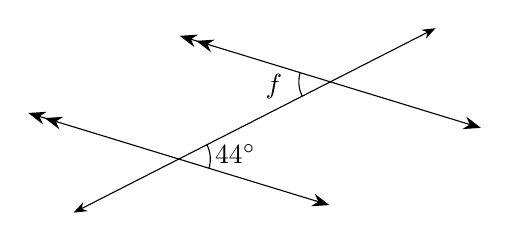
\begin{tikzpicture}[scale=1.0, baseline=(current bounding box.north)]
    \begin{scope}[rotate=27]
      % Draw the first line
      \draw[<->>, >={Stealth[scale=1.3]}, name path=P1] (0, 0) -- (-2.877359201354605, 2.7786334818359886);
      % Draw the second line with the calculated offsets
      \draw[<->>, >={Stealth[scale=1.3]}, name path=P2] (2.15933480943859, 0) -- (-0.7180243919160154, 2.7786334818359886);
      % Draw the transversal through the middle of the parallel lines
      \draw[<->, >=Stealth, name path=P3] (-2.938679600677303, 1.3893167409179943) -- (2.220655208761287, 1.3893167409179943);
      
      \path [name intersections={of=P1 and P3,by=A}];
      \path [name intersections={of=P2 and P3,by=B}];

      % Draw the angle
      \coordinate (p1s) at (0, 0);
      \coordinate (p1e) at (-2.877359201354605, 2.7786334818359886);
      \coordinate (p2s) at (2.15933480943859, 0);
      \coordinate (p2e) at (-0.7180243919160154, 2.7786334818359886);
      \coordinate (ts) at (-2.938679600677303, 1.3893167409179943);
      \coordinate (te) at (2.220655208761287, 1.3893167409179943);

      % order for vertices go in anticlockwise order te--A--p1e
      \draw pic["$f$", draw=black, -, angle eccentricity=1.8, angle radius=0.4cm] {angle=p2e--B--ts};
\draw pic["$44^\circ$", draw=black, -, angle eccentricity=1.8, angle radius=0.4cm] {angle=p1s--A--te};

      % %% Point A
      % \draw pic["$a$", draw=black, -, angle eccentricity=1.5, angle radius=0.4cm] {angle=te--A--p1e};
      % \draw pic["$b$", draw=black, -, angle eccentricity=1.5, angle radius=0.4cm] {angle=p1e--A--ts};
      % \draw pic["$c$", draw=black, -, angle eccentricity=1.5, angle radius=0.4cm] {angle=ts--A--p1s};
      % \draw pic["$d$", draw=black, -, angle eccentricity=1.5, angle radius=0.4cm] {angle=p1s--A--te};
      
      % %%  Point B
      % \draw pic["$e$", draw=black, -, angle eccentricity=1.5, angle radius=0.4cm] {angle=te--B--p2e};
      % \draw pic["$f$", draw=black, -, angle eccentricity=1.5, angle radius=0.4cm] {angle=p2e--B--ts};
      % \draw pic["$g$", draw=black, -, angle eccentricity=1.5, angle radius=0.4cm] {angle=ts--B--p2s};
      % \draw pic["$h$", draw=black, -, angle eccentricity=1.5, angle radius=0.4cm] {angle=p2s--B--te};

    \end{scope}
  \end{tikzpicture}
\end{minipage}%
\hfill
\begin{minipage}{0.2\textwidth}
  \begin{align*}
    \angle \text{f} &= \text{44}^\circ
  \end{align*}
\end{minipage}
\vspace{1cm}\begin{minipage}{0.75\textwidth}
  \refstepcounter{minipagecount}
  \noindent{(\theminipagecount)}\quad
  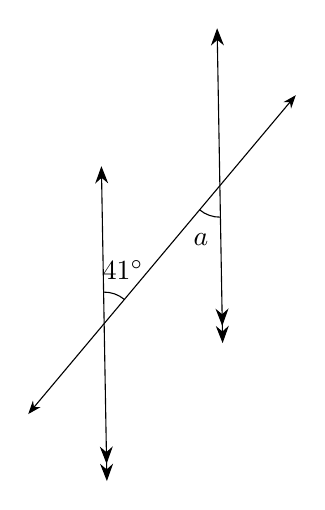
\begin{tikzpicture}[scale=1.0, baseline=(current bounding box.north)]
    \begin{scope}[rotate=230]
      % Draw the first line
      \draw[<->>, >={Stealth[scale=1.3]}, name path=P1] (0, 0) -- (3.018838320891088, 2.624236115962029);
      % Draw the second line with the calculated offsets
      \draw[<->>, >={Stealth[scale=1.3]}, name path=P2] (2.2863796300587214, 0) -- (5.305217950949809, 2.624236115962029);
      % Draw the transversal through the middle of the parallel lines
      \draw[<->, >=Stealth, name path=P3] (0.009419160445543806, 1.3121180579810146) -- (5.295798790504266, 1.3121180579810146);
      
      \path [name intersections={of=P1 and P3,by=A}];
      \path [name intersections={of=P2 and P3,by=B}];

      % Draw the angle
      \coordinate (p1s) at (0, 0);
      \coordinate (p1e) at (3.018838320891088, 2.624236115962029);
      \coordinate (p2s) at (2.2863796300587214, 0);
      \coordinate (p2e) at (5.305217950949809, 2.624236115962029);
      \coordinate (ts) at (0.009419160445543806, 1.3121180579810146);
      \coordinate (te) at (5.295798790504266, 1.3121180579810146);

      % order for vertices go in anticlockwise order te--A--p1e
      \draw pic["$a$", draw=black, -, angle eccentricity=1.8, angle radius=0.4cm] {angle=te--A--p1e};
\draw pic["$41^\circ$", draw=black, -, angle eccentricity=1.8, angle radius=0.4cm] {angle=ts--B--p2s};

      % %% Point A
      % \draw pic["$a$", draw=black, -, angle eccentricity=1.5, angle radius=0.4cm] {angle=te--A--p1e};
      % \draw pic["$b$", draw=black, -, angle eccentricity=1.5, angle radius=0.4cm] {angle=p1e--A--ts};
      % \draw pic["$c$", draw=black, -, angle eccentricity=1.5, angle radius=0.4cm] {angle=ts--A--p1s};
      % \draw pic["$d$", draw=black, -, angle eccentricity=1.5, angle radius=0.4cm] {angle=p1s--A--te};
      
      % %%  Point B
      % \draw pic["$e$", draw=black, -, angle eccentricity=1.5, angle radius=0.4cm] {angle=te--B--p2e};
      % \draw pic["$f$", draw=black, -, angle eccentricity=1.5, angle radius=0.4cm] {angle=p2e--B--ts};
      % \draw pic["$g$", draw=black, -, angle eccentricity=1.5, angle radius=0.4cm] {angle=ts--B--p2s};
      % \draw pic["$h$", draw=black, -, angle eccentricity=1.5, angle radius=0.4cm] {angle=p2s--B--te};

    \end{scope}
  \end{tikzpicture}
\end{minipage}%
\hfill
\begin{minipage}{0.2\textwidth}
  \begin{align*}
    \angle \text{a} &= \text{41}^\circ
  \end{align*}
\end{minipage}
\vspace{1cm}\begin{minipage}{0.75\textwidth}
  \refstepcounter{minipagecount}
  \noindent{(\theminipagecount)}\quad
  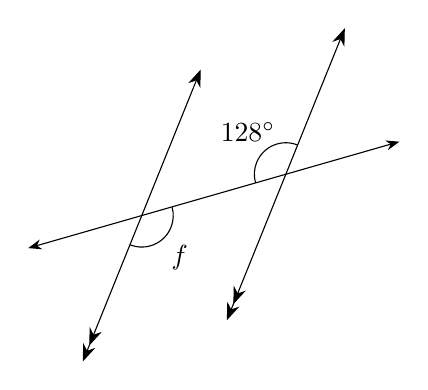
\begin{tikzpicture}[scale=1.0, baseline=(current bounding box.north)]
    \begin{scope}[rotate=196]
      % Draw the first line
      \draw[<->>, >={Stealth[scale=1.3]}, name path=P1] (0, 0) -- (2.462645901302633, 3.152043014426888);
      % Draw the second line with the calculated offsets
      \draw[<->>, >={Stealth[scale=1.3]}, name path=P2] (1.903527322608868, 0) -- (4.366173223911501, 3.152043014426888);
      % Draw the transversal through the middle of the parallel lines
      \draw[<->, >=Stealth, name path=P3] (-0.26867704934868364, 1.576021507213444) -- (4.634850273260184, 1.576021507213444);
      
      \path [name intersections={of=P1 and P3,by=A}];
      \path [name intersections={of=P2 and P3,by=B}];

      % Draw the angle
      \coordinate (p1s) at (0, 0);
      \coordinate (p1e) at (2.462645901302633, 3.152043014426888);
      \coordinate (p2s) at (1.903527322608868, 0);
      \coordinate (p2e) at (4.366173223911501, 3.152043014426888);
      \coordinate (ts) at (-0.26867704934868364, 1.576021507213444);
      \coordinate (te) at (4.634850273260184, 1.576021507213444);

      % order for vertices go in anticlockwise order te--A--p1e
      \draw pic["$f$", draw=black, -, angle eccentricity=1.8, angle radius=0.4cm] {angle=p2e--B--ts};
\draw pic["$128^\circ$", draw=black, -, angle eccentricity=1.8, angle radius=0.4cm] {angle=p1s--A--te};

      % %% Point A
      % \draw pic["$a$", draw=black, -, angle eccentricity=1.5, angle radius=0.4cm] {angle=te--A--p1e};
      % \draw pic["$b$", draw=black, -, angle eccentricity=1.5, angle radius=0.4cm] {angle=p1e--A--ts};
      % \draw pic["$c$", draw=black, -, angle eccentricity=1.5, angle radius=0.4cm] {angle=ts--A--p1s};
      % \draw pic["$d$", draw=black, -, angle eccentricity=1.5, angle radius=0.4cm] {angle=p1s--A--te};
      
      % %%  Point B
      % \draw pic["$e$", draw=black, -, angle eccentricity=1.5, angle radius=0.4cm] {angle=te--B--p2e};
      % \draw pic["$f$", draw=black, -, angle eccentricity=1.5, angle radius=0.4cm] {angle=p2e--B--ts};
      % \draw pic["$g$", draw=black, -, angle eccentricity=1.5, angle radius=0.4cm] {angle=ts--B--p2s};
      % \draw pic["$h$", draw=black, -, angle eccentricity=1.5, angle radius=0.4cm] {angle=p2s--B--te};

    \end{scope}
  \end{tikzpicture}
\end{minipage}%
\hfill
\begin{minipage}{0.2\textwidth}
  \begin{align*}
    \angle \text{f} &= \text{128}^\circ
  \end{align*}
\end{minipage}
\vspace{1cm}\begin{minipage}{0.75\textwidth}
  \refstepcounter{minipagecount}
  \noindent{(\theminipagecount)}\quad
  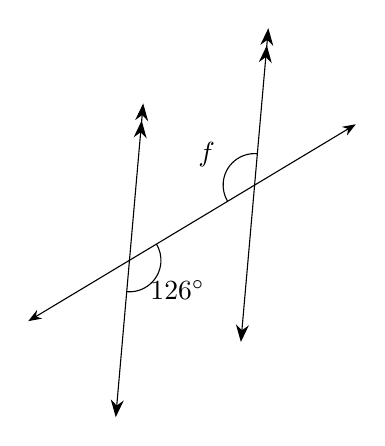
\begin{tikzpicture}[scale=1.0, baseline=(current bounding box.north)]
    \begin{scope}[rotate=31]
      % Draw the first line
      \draw[<->>, >={Stealth[scale=1.3]}, name path=P1] (0, 0) -- (2.3511410091698925, 3.23606797749979);
      % Draw the second line with the calculated offsets
      \draw[<->>, >={Stealth[scale=1.3]}, name path=P2] (1.8541019662496845, 0) -- (4.205242975419577, 3.23606797749979);
      % Draw the transversal through the middle of the parallel lines
      \draw[<->, >=Stealth, name path=P3] (-0.3244294954150537, 1.618033988749895) -- (4.529672470834631, 1.618033988749895);
      
      \path [name intersections={of=P1 and P3,by=A}];
      \path [name intersections={of=P2 and P3,by=B}];

      % Draw the angle
      \coordinate (p1s) at (0, 0);
      \coordinate (p1e) at (2.3511410091698925, 3.23606797749979);
      \coordinate (p2s) at (1.8541019662496845, 0);
      \coordinate (p2e) at (4.205242975419577, 3.23606797749979);
      \coordinate (ts) at (-0.3244294954150537, 1.618033988749895);
      \coordinate (te) at (4.529672470834631, 1.618033988749895);

      % order for vertices go in anticlockwise order te--A--p1e
      \draw pic["$f$", draw=black, -, angle eccentricity=1.8, angle radius=0.4cm] {angle=p2e--B--ts};
\draw pic["$126^\circ$", draw=black, -, angle eccentricity=1.8, angle radius=0.4cm] {angle=p1s--A--te};

      % %% Point A
      % \draw pic["$a$", draw=black, -, angle eccentricity=1.5, angle radius=0.4cm] {angle=te--A--p1e};
      % \draw pic["$b$", draw=black, -, angle eccentricity=1.5, angle radius=0.4cm] {angle=p1e--A--ts};
      % \draw pic["$c$", draw=black, -, angle eccentricity=1.5, angle radius=0.4cm] {angle=ts--A--p1s};
      % \draw pic["$d$", draw=black, -, angle eccentricity=1.5, angle radius=0.4cm] {angle=p1s--A--te};
      
      % %%  Point B
      % \draw pic["$e$", draw=black, -, angle eccentricity=1.5, angle radius=0.4cm] {angle=te--B--p2e};
      % \draw pic["$f$", draw=black, -, angle eccentricity=1.5, angle radius=0.4cm] {angle=p2e--B--ts};
      % \draw pic["$g$", draw=black, -, angle eccentricity=1.5, angle radius=0.4cm] {angle=ts--B--p2s};
      % \draw pic["$h$", draw=black, -, angle eccentricity=1.5, angle radius=0.4cm] {angle=p2s--B--te};

    \end{scope}
  \end{tikzpicture}
\end{minipage}%
\hfill
\begin{minipage}{0.2\textwidth}
  \begin{align*}
    \angle \text{f} &= \text{126}^\circ
  \end{align*}
\end{minipage}
\vspace{1cm}

\end{document}
